\documentclass[submit]{harvardml}

% You don't need to change these.
\course{CS181-S19}
\assignment{Assignment \#5}
\duedate{11:59pm April 19, 2019}
\newcommand{\attr}[1]{\textsf{#1}}
\usepackage[OT1]{fontenc}
\usepackage[colorlinks,citecolor=blue,urlcolor=blue]{hyperref}
\usepackage[pdftex]{graphicx}
\usepackage{subfig}
\usepackage{fullpage}
% \usepackage{palatino}
% \usepackage{mathpazo}
\usepackage{amsmath}
\usepackage{amssymb}
\usepackage{color}
\usepackage{todonotes}
\usepackage{listings}
\usepackage{common}
\usepackage{bm}
\usepackage{enumitem}
\usepackage{tikz}
\usepackage{xifthen}

\usepackage[mmddyyyy,hhmmss]{datetime}

\definecolor{verbgray}{gray}{0.9}

\lstnewenvironment{csv}{%
  \lstset{backgroundcolor=\color{verbgray},
  frame=single,
  framerule=0pt,
  basicstyle=\ttfamily,
  columns=fullflexible}}{}

\newcommand{\mueps}{\mu_{\epsilon}}
\newcommand{\sigeps}{\sigma_{\epsilon}}
\newcommand{\mugam}{\mu_{\gamma}}
\newcommand{\siggam}{\sigma_{\gamma}}
\newcommand{\muzp}{\mu_{p}}
\newcommand{\sigzp}{\sigma_{p}}
\newcommand{\gauss}[3]{\frac{1}{2\pi#3}e^{-\frac{(#1-#2)^2}{2#3}}}


\begin{document}
\begin{center}
{\Large Homework 5: Graphical Models, MDPs}\\
\end{center}

\subsection*{Introduction}

% FDV: Add useful readings here.

There is a mathematical component and a programming component to this
homework.  Please submit your \textbf{tex, PDF, and Python files} to
Canvas, and push all of your work to your GitHub repository. If a
question requires you to make any plots, please include those in the
writeup.

\newpage

\section*{Bayesian Networks [7 pts]}
\begin{problem}

  % FDV: Minor notation changes + changed the network.  Adjust the
  % solutions for the new network with the new names.

  \noindent In this problem we explore the conditional independence
  properties of a Bayesian Network.  Consider the following Bayesian
  network representing a student's work. Each random variable is
  binary (true/false).
 %
%\vspace{0.2in}
\begin{center}
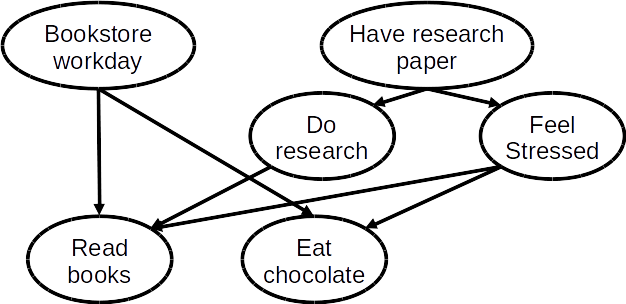
\includegraphics[width=3in]{bn.png}
\end{center}
%\vspace{0.2in}

The random variables are:
%
\begin{itemize}
\item \attr{Have research paper}: Does the student have a research paper?
\item \attr{Do Research}: Is the student doing research?
\item \attr{Feel Stressed}: Is the student feeling stressed?
\item \attr{Bookstore Workday}: Is the student working at the bookstore?
\item \attr{Read Books}: Is the student reading a book?
\item \attr{Eat Chocolate}: Is the student eating chocolate?
\end{itemize}

\medskip

For the following questions, $A \perp B$ means that events A and B are
independent and $A \perp B | C$ means that events A and B are independent
conditioned on C. Use the concept of d-separation to answer the
questions and show your work.

%
\begin{enumerate}
\item Is $\attr{Bookstore Workday} \perp \attr{Have research paper}$?
  If NO, give intuition for why.
%
%
\item Is $\attr{Bookstore Workday} \perp \attr{Have research
  paper}\given \attr{Read Books}$? If NO, give intuition for why.
%
%
\item Is $\attr{Do Research} \perp \attr{Eat Chocolate}$? If NO, give
  intuition for why.
%
\item Is $\attr{Do Research} \perp \attr{Eat Chocolate} \given
  \attr{Feel Stressed}$? If NO, give intuition for why.
%
\item Suppose the student has done some mindfulness exercises to avoid
  stress eating.  Now, when they are stressed, they read (fun) books
  but don't eat chocolate.  Draw the modified network.
%
%
\item For this modified network, is $\attr{Do Research} \perp
  \attr{Eat Chocolate}$? If NO, give an intuition why.  If YES,
  describe what observations (if any) would cause them to no longer be
  independent.
%
\end{enumerate}
\end{problem}
\subsection*{Solution}

\newpage

\section*{Kalman Filters [7 pts]}

% FDV: This problem is the same as last year.  Take a close look for
% anything that could have been confusing.

\begin{problem}
In this problem, you will implement a one-dimensional Kalman filter.
Assume the following dynamical system model:
  \begin{eqnarray*}
    z_{t+1} &= z_{t} + \epsilon_{t} \\
    x_{t} & = z_{t} + \gamma_{t}
  \end{eqnarray*}
  where $z$ are the hidden variables and $x$ are the observed
  measurements.  The random variables $\epsilon$ and $\gamma$ are
  drawn from the following Normal distributions:
  \begin{eqnarray*}
    \epsilon_t &\sim& N(\mueps,\sigeps) \\
    \gamma_t &\sim& N(\mugam,\siggam)
  \end{eqnarray*}
  where $\mueps = 0$, $\sigeps=0.05$, $\mugam = 0$ and $\siggam=1.0$

You are provided with the observed data $x$ and the hidden data $z$ in
\texttt{kf-data.csv}, and the prior on the first hidden state is $p(z_0)$ =
N($\muzp$,$\sigzp$) where $\muzp = 5$ and $\sigzp=1$

    \begin{enumerate}
      \item The distribution $p(z_t|x_0...x_t)$ will be Gaussian
        $N(\mu_t,\sigma^2_t)$. Derive an iterative update for the mean
        $\mu_t$ and variance $\sigma^2_t$ given the mean and variance
        at the previous time step ($\mu_{t-1}$ and $\sigma^2_{t-1}$).

       \item Implement this update and apply it to the observed data
         above (do not use the hidden data to find these
         updates). Provide a plot of $\mu_t$ over time as well as a
         $2\sigma_t$ interval around $\mu_t$ (that is $\mu_t \pm
         2\sigma_t$).  Does the Kalman filter ``catch up'' to the true
         hidden object?

       \item Repeat the same process but change the observation at
         time $t=10$ to $x_{t=10}=10.2$ (an extreme outlier
         measurement).  How does the Kalman filter respond to this
         outlier?

       \item Comment on the misspecification of dynamical system model
         for these data.  Based on the previous two parts, how does
         this misspecification affect the predictions?

\end{enumerate}
\end{problem}
\subsection*{Solution}

\newpage

% FDV: This problem is completely new, and will need solutions written
% out.  Please check carefully and suggest changes.  (Last year, this
% was a tricky concept, so while the computations below are easy it
% seemed to make sense to make it into a problem...)

\begin{problem}[Explaining Away, 7 pts]

  In this problem, you will carefully work out a basic example with
  the explaining away effect.  There are many derivations of this
  problem available in textbooks.  We emphasize that while you may
  refer to textbooks and other online resources for understanding how
  to do the computation, you should do the computation below from
  scratch, by hand.

  We have three binary variables, rain $r$, grass-wet $g$, and
  sprinkler $s$.  The conditional probability tables look like the
  following:
  \begin{eqnarray*}
    p(r = 1) &= 0.25 \\
    p(s = 1) &= 0.5 \\
    p(g = 1 | r = 0 , s = 0 ) &= 0 \\
    p(g = 1 | r = 1 , s = 0 ) &= .75 \\
    p(g = 1 | r = 0 , s = 1 ) &= .75 \\
    p(g = 1 | r = 1 , s = 1 ) &= 1
  \end{eqnarray*}

  \begin{enumerate}
    \item You check on the sprinkler without checking on the rain or
      the grass.  What is the probability that it is on?
    \item You notice it is raining and check on the sprinkler without
      checking the grass.  What is the probability that it is on?
    \item You notice that the grass is wet and go to check on the
      sprinkler (without checking if it is raining).  What is the
      probability that it is on?
    \item You notice that it is raining and the grass is wet.  You go
      check on the sprinkler.  What is the probability that it is on?
    \item What is the explaining away effect above?
    \end{enumerate}

\end{problem}

\subsection*{Solution}

\newpage

\begin{itemize}
    \item Name:
    \item Email:
    \item Collaborators:
    \item Approximately how long did this homework take you to complete (in hours):
\end{itemize}

\end{document}
